\documentclass[12pt]{article}
\usepackage{amsmath}
\usepackage{mathtools}
\usepackage{bigints}
\usepackage{parskip}
\usepackage{amssymb}

    \newenvironment{myindentpar}[1]%
     {\begin{list}{}%
             {\setlength{\leftmargin}{#1}}%
             \item[]%
     }
     {\end{list}}

\begin{document}
\title{Math for Bio Formula and Definitions Sheet}
\date{Spring 2014}
\author{}
\maketitle

\textbf{Distance Between Two Numbers:} 
\newline

\centerline{$d(x_{1},x_{2}) = |x_{2}-x_{1}| = |x_{1}-x_{2}|$}

\textbf{Midpoint Between Two Numbers:} 
\newline

\centerline{$m(x_{1},x_{2}) = \dfrac{1}{2} \cdot |x_{2}-x_{1}| = \dfrac{1}{2} \cdot |x_{1}-x_{2}|$}

\textbf{Distance Between Two Points:} 
\newline

\centerline{$d \Big((x_{1},y_{1}),(x_{2},y_{2}\Big) = \sqrt{(x_{2}-x_{1})^2+(y_{2}-y_{1})^2}$}

\textbf{Midpoint Between Two Points:} 
\newline

\centerline{$d \Big((x_{1},y_{1}),(x_{2},y_{2}\Big) =\Big(\dfrac{1}{2} \cdot (x_{1}+x_{2}), \dfrac{1}{2} \cdot (y_{1}+y_{2})\Big)$}

\textbf{Standard Equation for a Circle:} 
\newline

\centerline{$(x-h)^2+(y-k)^2=r^2$}
\vspace{.5cm}
\centerline{\textbf{Center:} $(h,k)$ \hspace{2cm} \textbf{Radius:} $\sqrt{r}$}

\newpage
{\bf \underline{Symmetries}}

\begin{myindentpar}{1cm}
\textbf{Y-Axis Symmetry} - symmetrical about the y-axis. Graphically, you could reflect the function over the y-axis and it would remain the same. Some examples of functions with y-axis symmetry are $y=x^2$ and $x^2+y^2=r^2$ (a circle centered at the origin)

\textbf{X-Axis Symmetry} - symmetrical about the x-axis. Graphically, you could reflect the function over the x-axis and it would remain the same. Some examples of functions with x-axis symmetry include $x=y^2$ and $x^2+y^2=r^2$

\textbf{Origin Symmetry} - symmetrical about the origin. Graphically, you could rotate the function 180 degrees about the origin and it would remain the same. Some examples include $y=x^3$ and $x^2+y^2=r^2$
\end{myindentpar}


{\bf \underline{Even \& Odd Functions}}
\begin{myindentpar}{1cm}
\textbf{Even Function} - a function is \textit{even} if $f(-x) = f(x)$ Even functions always have y-axis symmetry

\textbf{Odd Function} - a function is \textit{odd} if $f(-x) = -f(x)$ Odd functions always have origin symmetry
\end{myindentpar}

{\bf \underline{Intercepts}}
\begin{myindentpar}{1cm}
\textbf{Y-intercept} - the point where a graph passes through the y-axis. To find the y-intercept we set $x=0$ and solve for $y$

\textbf{X-intercept} - the point where a graph passes through the x-axis. To find the x-intercept we set $y=0$ and solve for $x$
\end{myindentpar}
\newpage
\textbf{Domain} - the set of numbers that you can input into your function

\begin{myindentpar}{1cm}
\textbf{Note:} Usually you need to be careful of two types of functions: 

\begin{enumerate}
\item \textbf{square root function} 

The function $f(x) = \sqrt{x}$ has a domain $x \geq 0$. 

You may also see something like $f(x) = \sqrt{(x-1)(5-x)(x+7)}$ and be asked to find the domain. 

You then need to solve $(x-1)(5-x)(x+7) \geq 0$ to find the domain
\item \textbf{rational function}

 A rational function is of the form $f(x) = \dfrac{P(x)}{Q(x)}$ where $P(x)$ and $Q(x)$ are polynomial. The domain of a rational function is all reals except for $Q(x)=0.$ 

For example the domain of $f(x) = \dfrac{x^2+3x+1}{x-1}$ is $(-\infty, 1) \cup (1, \infty)$
\end{enumerate}

 Sometimes you might see a combination of both. 

For example, find the domain of $f(x) = \dfrac{1}{\sqrt{(3-x)(2+x)}}$ We do this by solving $(3-x)(2+x)>0$
\end{myindentpar}

Graphically, you can determine the domain by scanning along the x-axis and seeing what x-values the function is not defined for.

\textbf{Range} - the set of numbers that are output from a function. Often harder to determine than the domain, we can determine the range graphically by scanning along the y-axis and seeing what y-values the function is not defined for.
\newpage


\textbf{Slope of a Line: } Given two different points $(x_{1},y_{1})$ and $(x_{2}, y_{2})$ the \textit{slope} of the line connecting these two points is given by
\newline

\centerline{$m = \dfrac{y_{2} - y_{1}}{x_{2}-x_{1}}$}
\vspace{.5cm}

\textbf{Point-Slope Equation of a Line:} The line with slope $m$ passing through $(x_{1}, y_{1})$ is given by
\newline

\centerline{$y - y_{1} = m(x-x_{1})$}
\vspace{.5cm}

\textbf{Slope Intercept Equation of a Line:} The line with slope $m$ has a slope-intercept form of 
\newline

\centerline{$y = mx+b$ \hspace{1cm} where b is the y-intercept}

\textbf{Parallel Lines:} two lines are parallel if they have the same slope

\textbf{Perpendicular Lines:} two lines are perpendicular if the slope of one line is the \textbf{negative reciprocal} of the slope of the other line

\textbf{Quadratic Function:} 
\newline

\centerline{$y = ax^2+bx+c$ \hspace{1cm} $a \neq 0$}
\vspace{.5cm}

\textbf{Vertex-Form of a Quadratic Function:} 
\newline

\centerline{$y = a(x-v_{1})^2+v_{2}$}

where $(v_{1},v_{2})$ is the $x,y$ coordinate of the vertex. We've also called this the standard form of a quadratic function
\newpage

\textbf{Quadratic Formula:} 
\newline

\centerline{$x = \dfrac{-b \pm \sqrt{b^2-4ac}}{2a}$}

\textbf{Vertical Shifts:} Let $c>0$

\begin{enumerate}
\item $y=f(x) + c$ shifts $f(x)$ c units up
\item $y=f(x) - c$ shifts $f(x)$ c units down
\end{enumerate}

\textbf{Horizontal Shifts:} Let $c>0$

\begin{enumerate}
\item $y=f(x+c)$ shifts $f(x)$ c units left
\item $y=f(x-c)$ shifts $f(x)$ c units right
\end{enumerate}

\textbf{Reflections:} 

\begin{enumerate}
\item $y=-f(x)$ reflects $f(x)$ about the x-axis
\item $y=f(-x)$ reflects $f(x)$ about the y-axis
\end{enumerate}

\textbf{Vertical Stretch \& Shrink:} 
\newline

\centerline{Let $c>0$. We consider $y=cf(x)$}

\begin{enumerate}
\item $c>1 \hspace{.75cm} \to$ stretch $f(x)$ vertically by a factor of c
\item $0<c<1 \to$ shrink $f(x)$ vertically by a factor of c
\end{enumerate}
\vspace{.5cm}
\textbf{Horizontal Stretch \& Shrink:} 
\newline

\centerline{Let $c>0$. We consider $y=f(cx)$}

\begin{enumerate}
\item $c>1 \hspace{.75cm} \to$ shrink $f(x)$ horizontally by a factor of c
\item $0<c<1 \to$ stretch $f(x)$ horizontally by a factor of c
\end{enumerate}

\newpage
\textbf{Graph of $\mathbf{y=x^2}$}

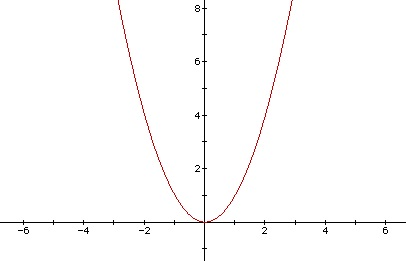
\includegraphics{Quadratic.jpg}

\textbf{Graph of $\mathbf{y=|x|}$}

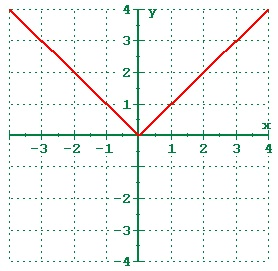
\includegraphics{AbsoluteValue.jpg}

\textbf{Note:} Remember the following two properties when solving absolute value inequalities:

\begin{enumerate}
\item $|x| < a \implies -a < x < a$
\item $|x| > a \implies x<-a$ and  $x>a$
\end{enumerate}

\textbf{Graph of $\mathbf{y=\sqrt{x}}$}

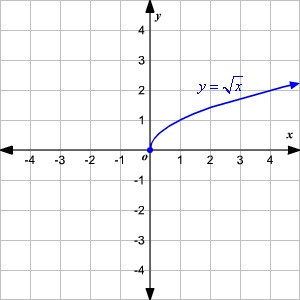
\includegraphics{SquareRoot.jpg}

\textbf{Arithmetic Combinations of Functions:}

\begin{enumerate}
\item $(f+g)(x) = f(x) + g(x)$
\begin{myindentpar}{1cm}
\textbf{Example:} Let $f(x) = x^2+3x+7$ and $g(x) = -x+2$

Then $(f+g)(x) =  (x^2+3x+7) + (-x+2) = x^2+2x+9$

\end{myindentpar}
\item $(f-g)(x) = f(x) - g(x)$

\begin{myindentpar}{1cm}
\textbf{Example:} Let $f(x) = x^2+3x+7$ and $g(x) = -x+2$

Then $(f+g)(x) =  (x^2+3x+7) - (-x+2) = x^2+4x+5$

\end{myindentpar}

\item $(f \cdot g)(x) = f(x) \cdot g(x)$
\begin{myindentpar}{1cm}
\textbf{Example:} Let $f(x) = x^2$ and $g(x) = \dfrac{1}{x}$

Then $(f \cdot g)(x) =  (x^2) \cdot \Big(\dfrac{1}{x}\Big) = \dfrac{x^2}{x} = x$

\end{myindentpar}
\newpage
\item $(\dfrac{f}{g})(x) = \dfrac{f(x)}{g(x)}$

\begin{myindentpar}{1cm}
\textbf{Example:} Let $f(x) = x^2+3x$ and $g(x) = \dfrac{1}{x^2}$

Then $(\dfrac{f}{g})(x) =  \dfrac{x^2+3x}{\dfrac{1}{x^2}} = x^2(x^2+3x) = x^4+3x^3$

\end{myindentpar}
\end{enumerate}

\textbf{Function Composition:} 

$(f \circ g)(x) = f \Big(g(x)\Big)$
\begin{myindentpar}{1cm}


\textbf{Example:} Let $f(x) = 3x^2-2$ and $g(x) = \dfrac{x+2}{x-1}$ 

Then $f \circ g = 3 \Big(\dfrac{x+2}{x-1} \Big)^2 -2$

\textbf{Note:} Be careful when finding the domain of a composition of functions. 
\end{myindentpar}
\begin{myindentpar}{2cm}
\textbf{Example:} Let $f(x) = \sqrt{x-12}$ and $g(x) = x^2-4$

Find 

a) $f \circ g$ 

b) $g \circ f$ 

and state the domain of each
\end{myindentpar}
\begin{myindentpar}{2.5cm}
\textbf{Answer:}
 \textbf{a)} $f \circ g = \sqrt{(x^2-4)-12}$

\hspace{3.3cm} $ = \sqrt{x^2-16}$

\textbf{Domain:} $x^2 - 16 \geq 0 \implies x\leq -4$ and $x \geq 4$

So the domain in interval notation is $(-\infty, -4] \cup [4, \infty)$

\textbf{Answer: b)} $g \circ f = \Big(\sqrt{x-12}\Big)^2 -4$

\hspace{3.3cm} $ = x-12 -4$

\hspace{3.3cm} $ = x-16$

\textbf{Domain:} $x - 12 \geq 0 \implies x \geq  12 \implies [12 , \infty)$
\end{myindentpar}

\textbf{One-to-One:} - a function is one-to-one if $f(x_{1}) = f(x_{2})$ implies $ x_{1}  = x_{2}$

\begin{myindentpar}{1cm}
\textbf{Horizontal Line Test:} - a nice, easy, graphical test to determine if a function is one-to-one. It says that a function is \textbf{one-to-one} if every horizontal line intersects a graph \textbf{at most once}

\textbf{Function That Passes the Horizontal Line Test:}

\centerline{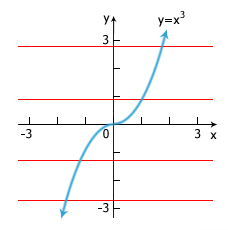
\includegraphics{PassHLT.jpg}}

\textbf{Function That Fails Horizontal Line Test:}

\centerline{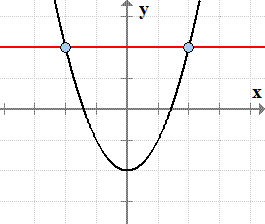
\includegraphics{FailHLT.png}}

\end{myindentpar}
\newpage
\textbf{Inverse Function:} - if a function $f$ is one-to-one then the \textbf{inverse function} denoted by $f^{-1}(x)$ is the function that "undoes" the original function $f$ so that $f^{-1}\Big(f(x)\Big) = x$ 

\begin{itemize}
\item The domain of $f$ is the range of $f^{-1}$
\item The range of $f$ is the domain of $f^{-1}$
\item Graphically, the inverse function, $f^{-1}(x)$, is the graph of the original function, $f(x)$,  reflected about the line $y=x$
\end{itemize}

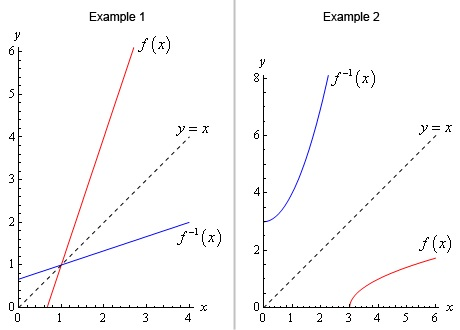
\includegraphics{InverseGraph.jpg}

\textbf{Note:} Notice how in Example 2 that the range of $f^{-1}(x)$ is the domain of $f(x)$

\textbf{Finding the Inverse Function:}

\begin{enumerate}
\item Set $y = f(x)$
\item Solve for $x$ in terms of $y$
\item Swap $x$ and $y$
\item Done!
\end{enumerate}











\end{document}